%------------------------------------------------
\begin{frame}
 \frametitle{Bunch-selective spin manipulation $\rightarrow$ co-magnetometry I}
 \framesubtitle{\textbf{World-first (September 2020 JEDI, with $d$ at \SI{970}{MeV/c})} \textcolor{PineGreen}{\cite{Slim:2023lpd,Nikolaev:2023srx}}}

\vspace{-0.25cm}
\begin{columns}[c]
\column{0.4\textwidth} 
\begin{center}
 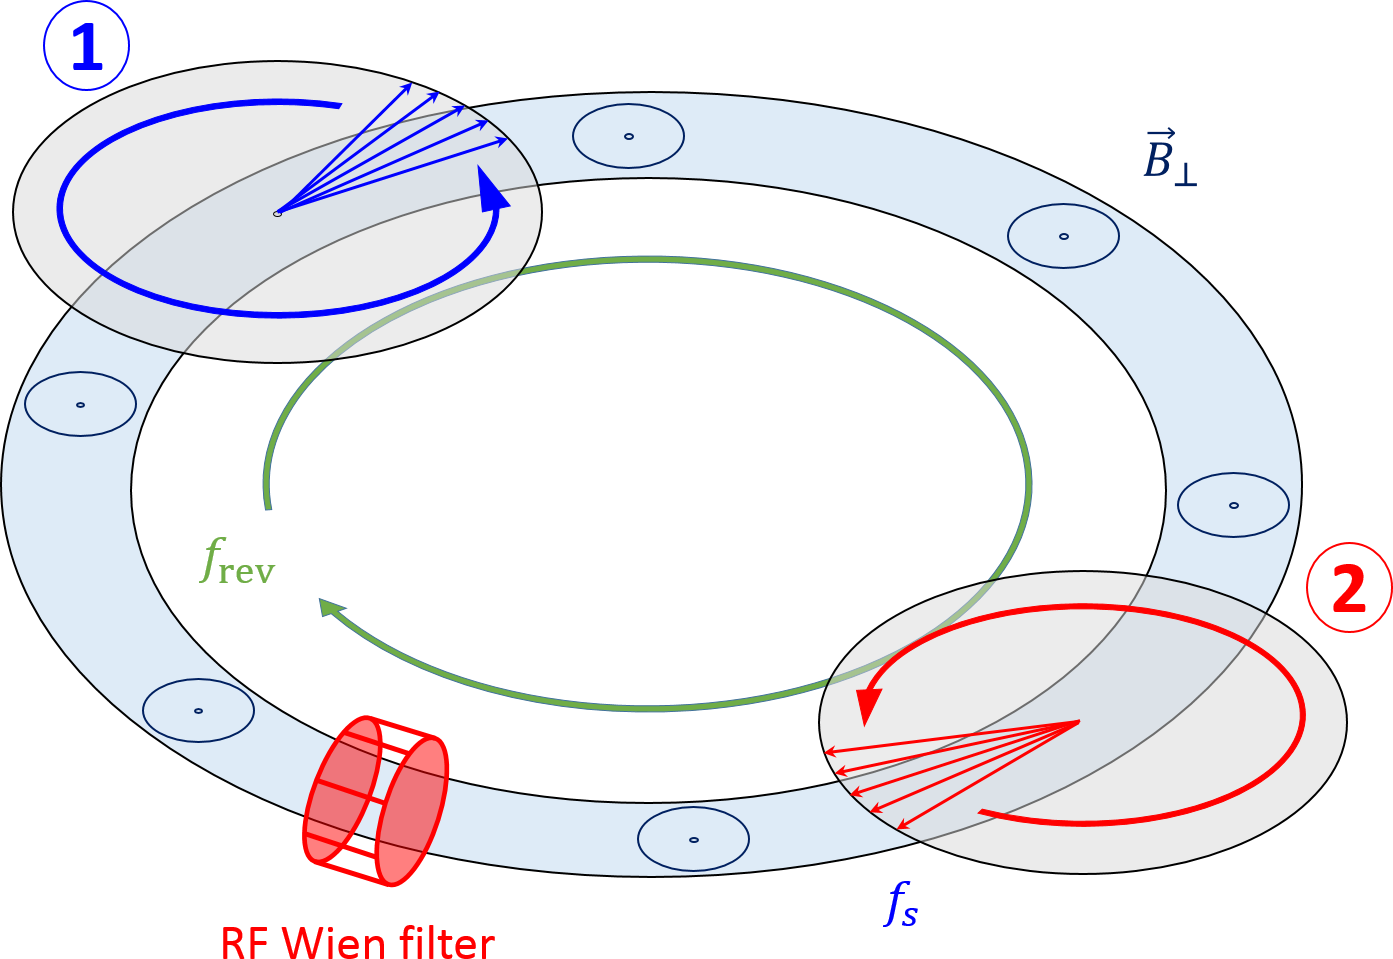
\includegraphics[height = 0.27\textheight]{spin-precession-3.png} 
\end{center}
 
\column{0.6\textwidth} 
\begin{small}
	\vspace{-0.25cm}
   \begin{itemize}
      \item signal\,\textcolor{blue}{\circled{\textbf{1}}} and pilot bunches\,\textcolor{red}{\circled{\textbf{2}}}:
      \begin{itemize}
          \item spin-coherent ensembles in ring plane orbit at $f_\text{rev} \approx \SI{750}{kHz}$
          \item precessing at $f_s \approx \SI{120}{kHz}$ 
      \end{itemize}
      \item waveguide RF WF\,\textcolor{PineGreen}{\cite{Slim2016116}} (\textit{radial} field $\vec B_r$), kept on resonance\footnotemark in\,\textcolor{blue}{\circled{\textbf{1}}} by spin tune measured in\,\textcolor{red}{\circled{\textbf{2}}}
   \end{itemize}
\end{small}
\end{columns}

\vspace{0.2cm}
\begin{small}
\textbf{\textit{Selective} gating of one of the two stored bunches at RF Wien filter: }
      \begin{itemize}
       \item[\textcolor{blue}{\circled{\textbf{1}}}] RF WF enhancement of  $p_y(t)$ of \textcolor{blue}{signal bunch}
       \item[\textcolor{red}{\circled{\textbf{2}}}] \textcolor{red}{pilot bunch}, unperturbed by RF WF, acts as co-magnetometer
      \end{itemize}
\end{small}

\footnotetext[1]{$f_{\mathrm{WF}}  =   K\cdot f_\text{rev} + f_s = (K + \nu_s)f_\text{rev}$, where $K \in \mathbb{Z}$ and  $\nu_s$ spin tune, $f_\text{WF}^{(K=-1)} \approx  \SI{871.431}{kHz}$} 

\vspace{-0.6cm}
\begin{columns}[T]
\column{0.48\textwidth} 
\begin{center}
   \includegraphics[height = 0.28\textheight]{bunches2DNorm_19082023.pdf} 
\end{center}


\column{0.48\textwidth} 
\begin{center}
    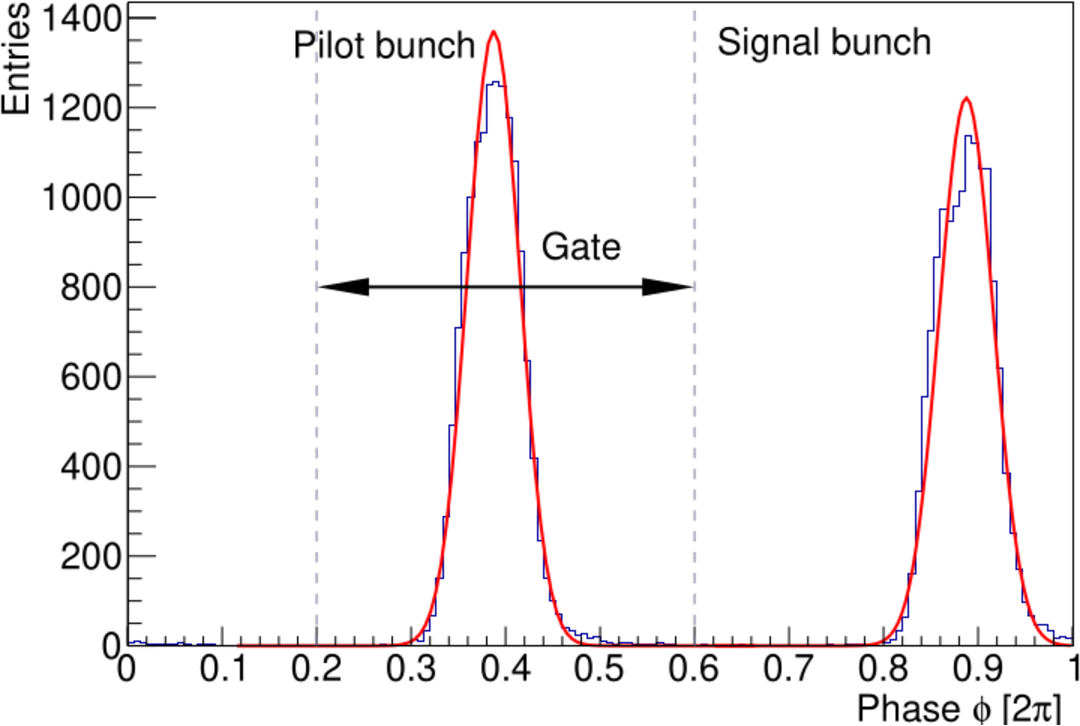
\includegraphics[height = 0.28\textheight]{bunches122_19082023.pdf} 
\end{center}

\end{columns}
 
\end{frame}
